\documentclass[aspectratio=169,11pt]{beamer}
\usetheme{Madrid}
\usecolortheme{default}
\usepackage{booktabs,graphicx,amsmath,tikz,xcolor}
\usetikzlibrary{arrows.meta,positioning}
\setbeamertemplate{navigation symbols}{}

% If the folder layout differs, change this path (see report.tex)
\newcommand{\resdir}{../results}
\input{\resdir/numbers.tex}
\newcommand{\todo}[1]{\textcolor{red}{[TODO: #1]}}
\newcommand{\figorbox}[2]{\IfFileExists{#1}{\includegraphics[#2]{#1}}{\fbox{\parbox{0.8\linewidth}{\centering Figure missing -- run the notebook}}}}

\title[Optimizers for CNNs]{A Comparative Study of Optimization Algorithms\\for CNN-Based Image Classification}
\subtitle{AI Deep Learning Lab -- Milestone 2 (Experimentation-Based)}
\author[V. Mitesh K.]{Vataliya Mitesh Kiritbhai (AU2644030)}
\institute[M.Tech CSE]{M.Tech CSE \\ \todo{Institution}}
\date[Nov 2026]{16 / 18 November 2026}

\begin{document}
\begin{frame}\titlepage\end{frame}

\begin{frame}{1. Problem Statement}
\begin{itemize}
  \item CNNs are the standard approach for image classification.
  \item Accuracy depends on the \textbf{optimizer} as well as the architecture: it controls convergence speed, generalisation and training cost.
  \item No optimizer is universally best~\footnotemark, so we compare them \emph{empirically} and \emph{fairly}.
\end{itemize}
\vspace{4pt}
\begin{block}{Research question}
Under identical training conditions, how do SGD, Adam, RMSprop and AdamW differ in accuracy, convergence behaviour and training time on CIFAR-10?
\end{block}
\footnotetext{Wilson et al., ``The Marginal Value of Adaptive Gradient Methods in ML'', NeurIPS 2017.}
\end{frame}

\begin{frame}{2. Objectives}
\begin{enumerate}
  \item Implement a CNN for CIFAR-10 in PyTorch.
  \item Train it with SGD, Adam, RMSprop and AdamW under controlled conditions.
  \item Evaluate accuracy, precision, recall and F1-score.
  \item Analyse loss curves and convergence speed.
  \item Compare training time / computational efficiency.
  \item Run a learning-rate sensitivity ablation.
  \item Identify the best optimizer for this setup.
\end{enumerate}
\end{frame}

\begin{frame}{3. System Architecture (Experiment Pipeline)}
\centering
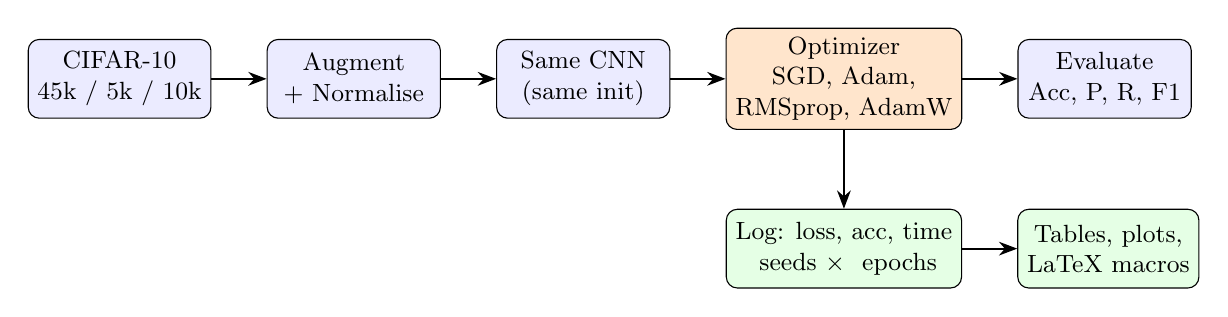
\begin{tikzpicture}[node distance=7mm, every node/.style={font=\small},
  box/.style={draw, rounded corners, fill=blue!8, minimum height=10mm, minimum width=22mm, align=center},
  arr/.style={-{Stealth}, thick}]
  \node[box] (d) {CIFAR-10\\45k / 5k / 10k};
  \node[box, right=of d] (a) {Augment\\+ Normalise};
  \node[box, right=of a] (m) {Same CNN\\(same init)};
  \node[box, right=of m, fill=orange!20] (o) {Optimizer\\SGD, Adam,\\RMSprop, AdamW};
  \node[box, right=of o] (e) {Evaluate\\Acc, P, R, F1};
  \draw[arr] (d)--(a); \draw[arr] (a)--(m); \draw[arr] (m)--(o); \draw[arr] (o)--(e);
  \node[box, below=10mm of o, fill=green!10] (l) {Log: loss, acc, time\\\nSeeds{} seeds $\times$ \nEpochs{} epochs};
  \draw[arr] (o)--(l);
  \node[box, right=of l, fill=green!10] (r) {Tables, plots,\\LaTeX macros};
  \draw[arr] (l)--(r);
\end{tikzpicture}

\vspace{6pt}
\small Tools: Python, PyTorch, Torchvision, scikit-learn, Matplotlib, Google Colab (GPU)
\end{frame}

\begin{frame}{4. Dataset: CIFAR-10}
\begin{columns}[T]
\column{0.55\textwidth}
\begin{itemize}
  \item 60,000 colour images, $32\times32\times3$, 10 classes (6,000 each)
  \item Official split: 50,000 train / 10,000 test
  \item Our split: \textbf{45,000 train / 5,000 validation} (fixed seed) / 10,000 test
  \item Train augmentation: random crop (pad 4) + horizontal flip
  \item Per-channel mean/std normalisation
\end{itemize}
\column{0.4\textwidth}
\small airplane, automobile, bird, cat, deer, dog, frog, horse, ship, truck
\vspace{6pt}

\begin{alertblock}{No test leakage}
Test set is used only once, for the best-validation checkpoint.
\end{alertblock}
\end{columns}
\end{frame}

\begin{frame}{5. Model: Custom CNN (\nParams{} parameters)}
\centering
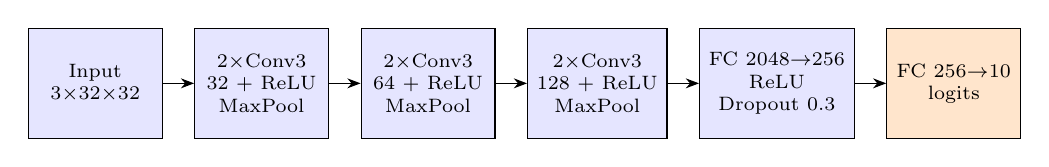
\begin{tikzpicture}[every node/.style={font=\scriptsize}, b/.style={draw, fill=blue!10, minimum height=14mm, minimum width=17mm, align=center}, arr/.style={-{Stealth}}]
  \node[b] (i) {Input\\$3{\times}32{\times}32$};
  \node[b, right=4mm of i] (c1) {2$\times$Conv3\\32 + ReLU\\MaxPool};
  \node[b, right=4mm of c1] (c2) {2$\times$Conv3\\64 + ReLU\\MaxPool};
  \node[b, right=4mm of c2] (c3) {2$\times$Conv3\\128 + ReLU\\MaxPool};
  \node[b, right=4mm of c3] (f) {FC 2048$\to$256\\ReLU\\Dropout 0.3};
  \node[b, right=4mm of f, fill=orange!20] (o) {FC 256$\to$10\\logits};
  \foreach \a/\b in {i/c1,c1/c2,c2/c3,c3/f,f/o} \draw[arr] (\a)--(\b);
\end{tikzpicture}

\vspace{8pt}
\begin{itemize}
  \item Deliberately small, so differences come from the \textbf{optimizer}, not the architecture.
  \item Identical architecture, initial weights (per seed) and mini-batch order for every optimizer.
\end{itemize}
\end{frame}

\begin{frame}{6. Experimental Design}
\centering\small
\begin{tabular}{lll}
\toprule
\textbf{Optimizer} & \textbf{Role} & \textbf{Settings}\\
\midrule
SGD & Baseline & $\eta{=}0.01$, momentum 0.9\\
Adam & Comparison & $\eta{=}10^{-3}$, $\beta{=}(0.9,0.999)$\\
RMSprop & Comparison & $\eta{=}10^{-3}$, $\alpha{=}0.99$\\
AdamW & Comparison & $\eta{=}10^{-3}$, weight decay $10^{-2}$\\
\bottomrule
\end{tabular}

\vspace{8pt}
\raggedright
\begin{itemize}
  \item \textbf{Fixed:} data split, augmentation, loss (cross-entropy), batch size 128, \nEpochs{} epochs, evaluation
  \item \textbf{Repeats:} \nSeeds{} seeds per optimizer $\Rightarrow$ mean $\pm$ std
  \item \textbf{Metrics:} accuracy, macro precision/recall/F1, loss, epochs to \convThresh\% val.\ accuracy, training time
\end{itemize}
\end{frame}

\begin{frame}{7. Results: Test Performance}
\centering
\resizebox{\linewidth}{!}{\IfFileExists{\resdir/results_table.tex}{\input{\resdir/results_table.tex}}{\fbox{run the notebook}}}

\vspace{8pt}
\raggedright
\begin{itemize}
  \item Best mean accuracy: \textbf{\bestOpt} (\bestAcc\,\% $\pm$ \bestAccStd); lowest: \worstOpt{} (\worstAcc\,\%)
  \item Gap between best and worst: \accGap{} percentage points
  \item \todo{Is the gap larger than the seed-to-seed std? Say so honestly.}
\end{itemize}
\end{frame}

\begin{frame}{8. Results: Convergence}
\centering
\figorbox{\resdir/figures/loss_curves.pdf}{height=0.33\textheight}

\figorbox{\resdir/figures/val_acc_curves.pdf}{height=0.30\textheight}
\vspace{-2pt}
\begin{itemize}\small
 \item First to reach \convThresh\% validation accuracy: \fastConvOpt\quad \todo{one more observation from the curves}
\end{itemize}
\end{frame}

\begin{frame}{9. Results: Efficiency \& Class Behaviour}
\begin{columns}[T]
\column{0.58\textwidth}
\figorbox{\resdir/figures/accuracy_time_bars.pdf}{width=\linewidth}
\small Seconds per epoch: SGD \speSGD, Adam \speAdam, RMSprop \speRMSprop, AdamW \speAdamW. Fastest: \fastestOpt.\\ \todo{Are the differences meaningful?}
\column{0.4\textwidth}
\figorbox{\resdir/figures/confusion_matrix.pdf}{width=\linewidth}
\end{columns}
\end{frame}

\begin{frame}{10. Ablation: Learning-Rate Sensitivity}
\begin{columns}[T]
\column{0.5\textwidth}
\figorbox{\resdir/figures/lr_sensitivity.pdf}{width=\linewidth}
\column{0.48\textwidth}
\begin{itemize}\small
  \item 3 learning rates per optimizer, 1 seed, \sweepEpochs{} epochs
  \item Checks that the ranking is not an artefact of the chosen defaults
  \item \todo{Most / least LR-sensitive optimizer?}
\end{itemize}
\end{columns}
\end{frame}

\begin{frame}{11. Conclusion \& Future Work}
\begin{itemize}
  \item Controlled comparison of 4 optimizers, same CNN / data / budget, \nSeeds{} seeds each.
  \item \textbf{\bestOpt} gave the highest mean test accuracy: \bestAcc\,\%.
  \item \todo{Speed / stability takeaway and recommendation.}
\end{itemize}
\vspace{4pt}
\begin{block}{Limitations \& next steps}
Single small CNN and dataset, no LR schedule, defaults not tuned per optimizer. Next: LR schedules, ResNet, CIFAR-100, per-optimizer tuning.
\end{block}
\end{frame}


\end{document}
